% It is an example file showing how to use the 'sigkddExp.cls'
% LaTeX2e document class file for submissions to sigkdd explorations.
% It is an example which *does* use the .bib file (from which the .bbl file
% is produced).
% REMEMBER HOWEVER: After having produced the .bbl file,
% and prior to final submission,
% you need to 'insert'  your .bbl file into your source .tex file so as to provide
% ONE 'self-contained' source file.
%
% Questions regarding SIGS should be sent to
% Adrienne Griscti ---> griscti@acm.org
%
% Questions/suggestions regarding the guidelines, .tex and .cls files, etc. to
% Gerald Murray ---> murray@acm.org
%

\documentclass{sigkddExp}

\begin{document}
%
% --- Author Metadata here ---
% -- Can be completely blank or contain 'commented' information like this...
%\conferenceinfo{WOODSTOCK}{'97 El Paso, Texas USA} % If you happen to know the conference location etc.
%\CopyrightYear{2001} % Allows a non-default  copyright year  to be 'entered' - IF NEED BE.
%\crdata{0-12345-67-8/90/01}  % Allows non-default copyright data to be 'entered' - IF NEED BE.
% --- End of author Metadata ---

\title{Paper v0 draft}
%\subtitle{[Extended Abstract]
% You need the command \numberofauthors to handle the "boxing"
% and alignment of the authors under the title, and to add
% a section for authors number 4 through n.
%
% Up to the first three authors are aligned under the title;
% use the \alignauthor commands below to handle those names
% and affiliations. Add names, affiliations, addresses for
% additional authors as the argument to \additionalauthors;
% these will be set for you without further effort on your
% part as the last section in the body of your article BEFORE
% References or any Appendices.

\numberofauthors{5}
%
% You can go ahead and credit authors number 4+ here;
% their names will appear in a section called
% "Additional Authors" just before the Appendices
% (if there are any) or Bibliography (if there
% aren't)

% Put no more than the first THREE authors in the \author command
%%You are free to format the authors in alternate ways if you have more
%%than three authors.

\author{
%
% The command \alignauthor (no curly braces needed) should
% precede each author name, affiliation/snail-mail address and
% e-mail address. Additionally, tag each line of
% affiliation/address with \affaddr, and tag the
%% e-mail address with \email.
\alignauthor Ben Trovato \\
       \affaddr{Institute for Clarity in Documentation}\\
       \affaddr{1932 Wallamaloo Lane}\\
       \affaddr{Wallamaloo, New Zealand}\\
       \email{trovato@corporation.com}
\alignauthor G.K.M. Tobin\\
       \affaddr{Institute for Clarity in Documentation}\\
       \affaddr{P.O. Box 1212}\\
       \affaddr{Dublin, Ohio 43017-6221}\\
       \email{webmaster@marysville-ohio.com}
\alignauthor Lars Th{\o}rv\"{a}ld\titlenote{This author is the
one who did all the really hard work.}\\
       \affaddr{The Th{\o}rv\"{a}ld Group}\\
       \affaddr{1 Th{\o}rv\"{a}ld Circle}\\
       \affaddr{Hekla, Iceland}\\
       \email{larst@affiliation.org}
}
\additionalauthors{Additional authors: John Smith (The Th{\o}rvald Group,
email: {\texttt{jsmith@affiliation.org}}) and Julius P.~Kumquat
(The Kumquat Consortium, email: {\texttt{jpkumquat@consortium.net}}).}
\date{30 July 1999}
\maketitle
\begin{abstract}
In this section, we will ...
\end{abstract}


\section{Introduction}


...

\subsection{Score and KPIs}

we will briefly introduce introduce KPIs for monitoring the Data-Base System state...

health score is a overview estimation of current system state, which is computed according to expert's experience rule.

\subsection{Problem Definition}
  - multi-step forecast for score

making forecast on system's health score provides great convenience for operation work. (make decision in advance). We define it as univariate multi-step forecast task because the whole forecasting horizon offers both value and tendency. ....\begin{equation} x_{t+H}, x_{t+H-1}, ..., x_{t+1} = model({\cal C}_t; \Theta)\end{equation}

  - figure out main factors(among KPIs) for score $AND$ over score's forecasting horizon

health state(score) is currently summarized from Key Performance Indicators(KPIs). In different time interval, score is mainly affected by certain different KPIs called time-varying main factors. Figuring out the time-varying main factors of health score offers more details...In a time interval, a $kpi$ is though as one of main factors when its correlation with score is relative strong. Assuming that we have a correlation measurement $R(X, Y)$ for univariate time-series $X$ and $Y$, and time interval size is $W$. At time $t$, we can caculate $R(score[t-W+1:t], kpi^{i}[t-W+1:t])$ as $i-th$ kpi's correlation with score denoted as $R^{i}_{t}$. In fact, we want to get $R^{i}_{t}$ over score's forecasting horizon. Actually, making forecast on each kpi is impossible compared with score forecast...Instead of predicting the each forecasting step of $R^{i}_{t}$, we focus on the their mean value over score's forecasting horizon through looking back on history data of $R^{i}_{t}$.





The remainder of this document is ...

\section{FORMULATION AND MODEL}
In this section, we ...

\subsection{Framework Overview}
  - give a figure of the model framework

  - given a brief introduction for the process steps


\subsection{Multilevel Discrete Wavelets Transform}

  - MDWT's formulation

time-frequence analysis of signal process.
\begin{equation}x(t)=\sum_{k}c_{j_0}[k] \; \varphi_{j_0, k}(t)+\sum_{j=j_0}^{J}\sum_{k}d_{j}[k] \ \psi_{j,k}(t) \end{equation}
In the signal space consisting of and wavelet functions $\psi_{j,k}(t)$, ...

  - MDWT's advantage applied for time-seires forecasting task

pattern of score time-series can be captured DWT transform domain. (decomposing the task into sub-taks and training seperately can achieve better performance)

\subsection{seq2seq-based Forecast}
  - classic seq2seq model is build for NLP.
the model can map input sequence to ouput sequence

  - insight of seq2seq model when it is applied for multi-step forecasting task. the decoder component can be seen as State Space Model([Machine Learning for Spatiotemporal Sequence Forecasting: A Survey])

\subsection{Correlation Measurement and Prediction}
  - correlation measurement $R(X, Y)$ function as Pearson Correlation Coefficient (PCC)
Here, the modified PCC is computed as following.
\begin{equation}
R(X, Y) = \begin{cases}
0, \quad var(X)=0 || var(Y)=0 \\\\
PCC(X, Y), \quad else
\end{cases}
\end{equation}

  - Gated-RNN for predicting mean PCC over score's forecasting horizon using history PCC data.

\subsection{Joint Task}
  - Firtly, we must illustrate the relation between two task explicitly.

  - Secondly, explain why (sharing the latency represtative vector), (constructing universe loss function) and (training jointly) are effective theoretically.

\section{Experiments and Results}
In this section, we ...

\subsection{Data-Base Date Set}
  - discribe the source of the data set and its meaning

  - give a statistics of health score distribution, Fig. \ref{score distribution}.

  (a figure about frequency and cumulative probability, x-axis is score bins and y-axis is frequency, after we ignore the outlier, not in $[mean-3 \times std, mean+3 \times std], 99\%$)
\begin{figure}
  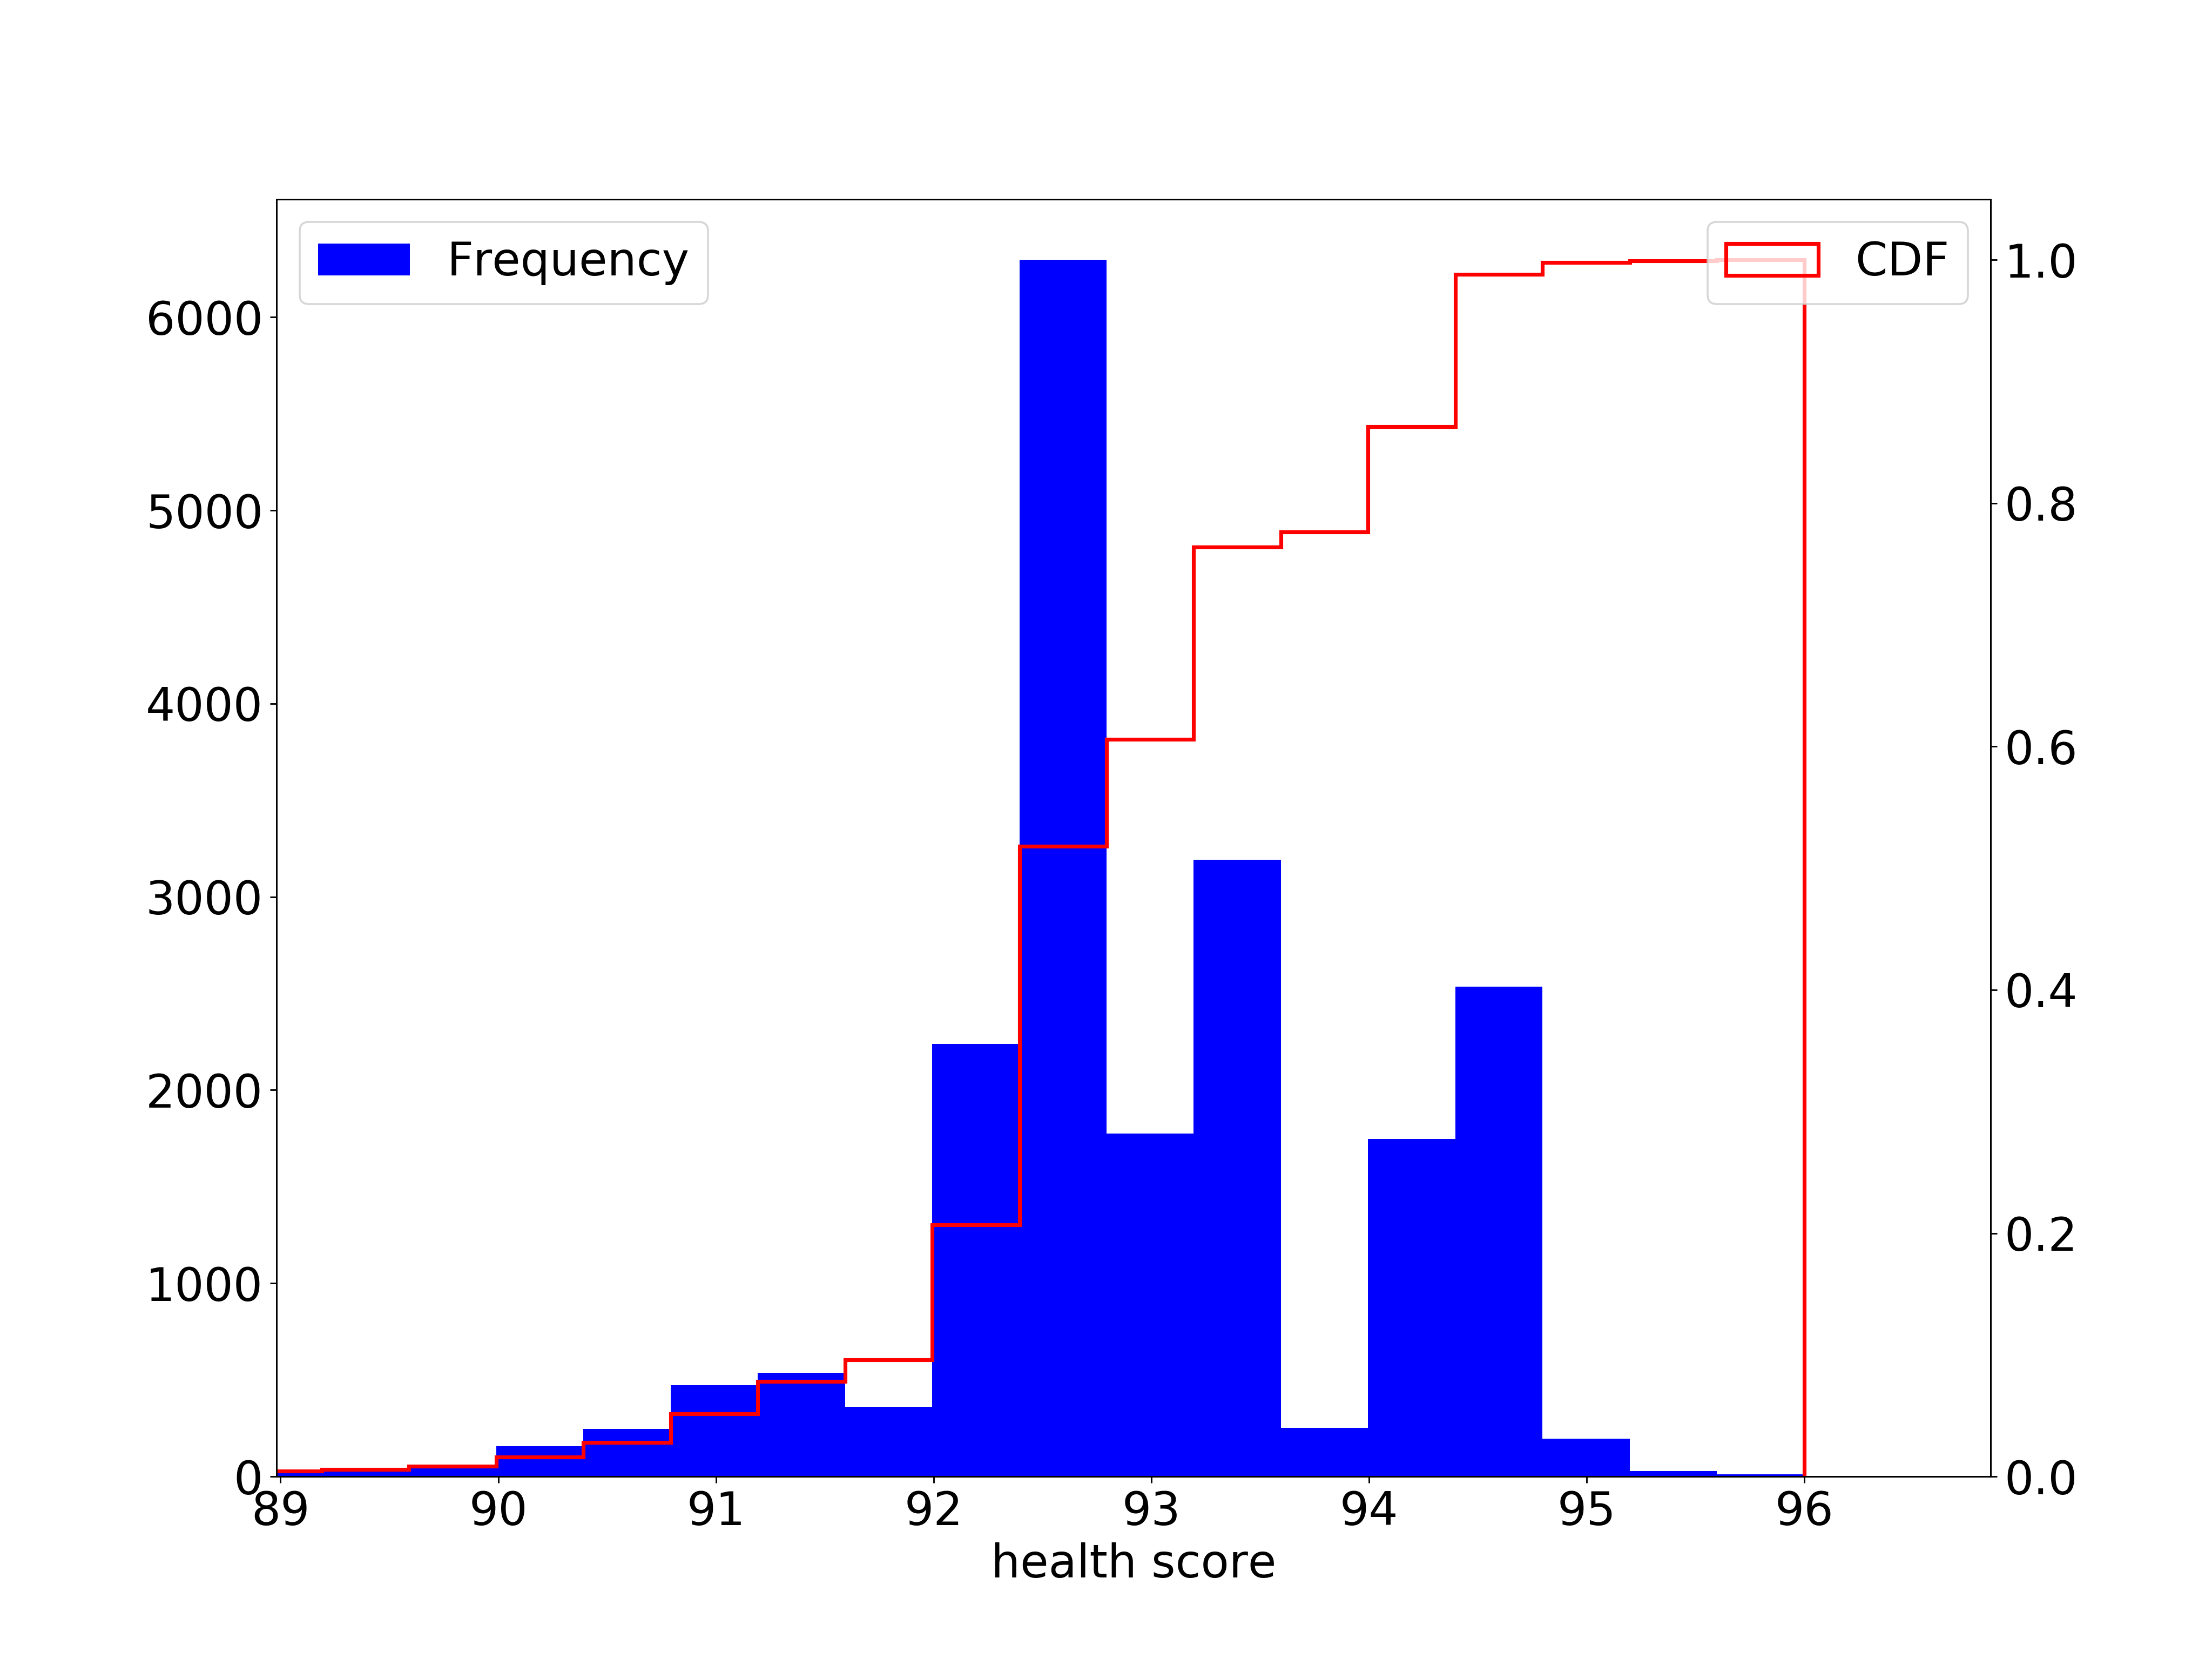
\includegraphics[width=0.48\textwidth]{Figures/showScoreDis.png}
  \caption{score distribution}
  \label{score distribution}
\end{figure}

  - give a figure about computed correlation between score and kpi, and illustrate correlation measurement's effectiveness.

\subsection{Task I: Score's Multi-step Forecast}

  - multi-forecast method includes baselie: AR or ARIMA, basic-LSTM, seq2seq, MDWT-based seq2seq (and its joint version). List the corresponding MAE and RMSE as a table.

  - MAE or RMSE's curve along with forecasting step' increase.

  - visualize the result vector over forecasting horizon, (try to find another evaluation measurement for multi-step forecasting model)

\subsection{Task II: correlation prediction}

  - mainly compare the seperate model and joint multi-task model (using correlation prediction RMSE or MAE, show that joint two relative task can improve model's performance....)

  - we can compute the (accuracy and recall) over Top M main factors, comparing seperate model and joint model and list the result as a table.


\section{Conclusions}
...

\section{Related Work}
...

\section{Acknowledgements}

%
% The following two commands are all you need in the
% initial runs of your .tex file to
% produce the bibliography for the citations in your paper.
\bibliographystyle{abbrv}
\bibliography{sigproc}  % sigproc.bib is the name of the Bibliography in this case
% You must have a proper ".bib" file
%  and remember to run:
% latex bibtex latex latex
% to resolve all references
%
% ACM needs 'a single self-contained file'!
%
%APPENDICES are optional
% SIGKDD: balancing columns messes up the footers: Sunita Sarawagi, Jan 2000.
% \balancecolumns
\appendix
%Appendix A
\section{Headings in Appendices}
The rules about hierarchical headings discussed above for
the body of the article are different in the appendices.
In the \textbf{appendix} environment, the command
\textbf{section} is used to
indicate the start of each Appendix, with alphabetic order
designation (i.e. the first is A, the second B, etc.) and
a title (if you include one).  So, if you need
hierarchical structure
\textit{within} an Appendix, start with \textbf{subsection} as the
highest level. Here is an outline of the body of this
document in Appendix-appropriate form:
\subsection{Introduction}
\subsection{The Body of the Paper}
\subsubsection{Type Changes and Special Characters}
\subsubsection{Math Equations}
\paragraph{Inline (In-text) Equations}
\paragraph{Display Equations}
\subsubsection{Citations}
\subsubsection{Tables}
\subsubsection{Figures}
\subsubsection{Theorem-like Constructs}
\subsubsection*{A Caveat for the \TeX\ Expert}
\subsection{Conclusions}
\subsection{Acknowledgements}
\subsection{Additional Authors}
This section is inserted by \LaTeX; you do not insert it.
You just add the names and information in the
\texttt{{\char'134}additionalauthors} command at the start
of the document.
\subsection{References}
Generated by bibtex from your ~.bib file.  Run latex,
then bibtex, then latex twice (to resolve references)
to create the ~.bbl file.  Insert that ~.bbl file into
the .tex source file and comment out
the command \texttt{{\char'134}thebibliography}.
% This next section command marks the start of
% Appendix B, and does not continue the present hierarchy
\section{More Help for the Hardy}
The acmproc-sp document class file itself is chock-full of succinct
and helpful comments.  If you consider yourself a moderately
experienced to expert user of \LaTeX, you may find reading
it useful but please remember not to change it.

% That's all folks!
\end{document}
